% =========================================================================
% BLOQUE II: RESULTADOS EXPERIMENTALES EN 5 ETAPAS Y SOTA (DIAPOSITIVAS 9 A 14)
% =========================================================================

% --- DIAPOSITIVA 9: MAPA GENERAL DE LAS CINCO ETAPAS EXPERIMENTALES ---
\begin{frame}{Mapa General de las Cinco Etapas Experimentales}{Trazabilidad de las 723 ejecuciones bajo preprocesamiento fijo \texttt{P0} \cite{rodas_valencia_tpe_ecog}}
  \scriptsize
  \begin{block}{Regla de Evaluaci\'on y Agregaci\'on Estrica (Sin \textit{Cherry-Picking})}
    La correlaci\'on de Pearson $r_{s,d} = \operatorname{corr}(\mathbf{y}_{s,d}, \hat{\mathbf{y}}_{s,d})$ se calcula sobre la \textbf{trayectoria continua completa} reconstruida mediante \textit{overlap-add} ($119$ ventanas sobre $N=7750$ muestras por bloque), promediando los $5$ dedos, los $5$ folds en CV y las \textbf{$3$ semillas completas en Test} (\texttt{3042, 4042, 5042}).
  \end{block}

  \vspace{1mm}
  \centering
  \renewcommand{\arraystretch}{1.22}
  \setlength{\tabcolsep}{4.5pt}
  \begin{tabular}{@{} l c c c c l @{}}
    \toprule
    \rowcolor{ipnDark}
    \textcolor{white}{\textbf{Etapa Experimental (\texttt{P0} fijo)}} &
    \textcolor{white}{\textbf{Sujeto 1}} &
    \textcolor{white}{\textbf{Sujeto 2}} &
    \textcolor{white}{\textbf{Sujeto 3}} &
    \textcolor{white}{\textbf{Media Global}} &
    \textcolor{white}{\textbf{Cambio / Interpretaci\'on Metodol\'ogica}} \\
    \midrule
    \textbf{1.\ \texttt{A0} Base (CV \'ep.\ 50)} & $0.4990$ & $0.4289$ & $0.7187$ & $\mathbf{0.5489}$ & Referencia inicial ($15$ entrenamientos). \\
    \rowcolor{rowLight}
    \textbf{2.\ \texttt{A5} sin TPE (CV \'ep.\ 50)} & $0.6038$ & $0.6216$ & $0.8258$ & $\mathbf{0.6837}$ & $\mathbf{+0.1349}$ por redise\~no arquitect\'onico ($14/15$ folds $>0$). \\
    \textbf{2b.\ \texttt{A5} sin TPE (\textit{Checkpoint*} ES)} & $0.7103$ & $0.6466$ & $0.8422$ & $\mathbf{0.7330}$ & $\mathbf{+0.0493}$ por selecci\'on temporal de \textit{checkpoint} (sin TPE). \\
    \rowcolor{rowLight}
    \textbf{3.\ \texttt{A5} con TPE (Mejor trial CV)} & $0.7117$ & $0.6878$ & $0.8533$ & $\mathbf{0.7509}$ & $\mathbf{+0.0179}$ en b\'usqueda ($32$ trials/sujeto $= 480$ fits). \\
    \textbf{4.\ \texttt{A5} Verificada (Nuevas semillas CV)} & $0.6929$ & $0.6785$ & $0.8402$ & $\mathbf{0.7372}$ & $\mathbf{+0.0041}$ neto global vs.\ 2b; $\mathbf{+0.0319}$ en \texttt{S2} ($60$ fits). \\
    \midrule
    \rowcolor{rowLight}
    \textbf{5a.\ \texttt{A5} Test Inicial (\texttt{B1--B4}, ES en \texttt{B5})} & $0.6087$ & $0.5226$ & $0.7685$ & $\mathbf{0.6333}$ & Primera evaluaci\'on en conjunto de prueba oficial ($9$ fits). \\
    \rowcolor{rowHighlight}
    \textbf{5b.\ \texttt{A5} Test Oficial (\texttt{B1--B5}, \'ep.\ fijas)} & $\mathbf{0.6723}$ & $\mathbf{0.5490}$ & $\mathbf{0.7796}$ & $\mathbf{0.6669}$ & $\mathbf{+0.0337}$ al reentrenar con el $100\%$ de desarrollo ($9/9 > 0$). \\
    \bottomrule
  \end{tabular}
\end{frame}

% --- DIAPOSITIVA 10: ETAPA 1 Y ETAPA 2: ABLACIONES Y SELECCIÓN DE CHECKPOINT ---
\begin{frame}{Etapas 1 y 2: Ablaciones Arquitect\'onicas y Selecci\'on de \textit{Checkpoint}}{Descomposici\'on del salto $\texttt{A0} \to \texttt{A5}$ ($+0.1349$) y efecto de la parada temprana ($+0.0493$)}
  \begin{columns}[T,onlytextwidth]
    \begin{column}{0.46\textwidth}
      \scriptsize
      \begin{block}{Hallazgos de la Campa\~na de Ablaci\'on ($165$ fits)}
        \begin{itemize}\setlength{\itemsep}{2.5pt}
          \item \textbf{Salto estructural $\texttt{A0} \to \texttt{A5}$ en \'epoca 50:} Sube de $0.5489$ a $\mathbf{0.6837}$ ($\mathbf{\Delta = +0.1349}$), positivo en \textbf{$14/15$ folds} (\texttt{S2} gana $\mathbf{+0.1927}$; \'unica excepci\'on \texttt{S1-B3} con $-0.0359$).
          \item \textbf{Sinergia multicomponente:} En \texttt{A3}, introducir \texttt{ConvTranspose1d} de forma aislada degrad\'o el modelo en $\mathbf{-0.0316}$ ($0.5173$). La ganancia emerge del acoplamiento con \texttt{LayerNorm} (\texttt{A1}: $+0.0605$), menor \texttt{Dropout} (\texttt{A2}) y fusi\'on previa del \textit{skip} (\texttt{A5b}: $0.6779 \to \texttt{A5}: 0.6837$).
        \end{itemize}
      \end{block}

      \begin{alertblock}{Puente Metodol\'ogico 2b: \textit{Checkpoint} Pre-TPE}
        Aplicar \textit{Early Stopping} ($\text{min}=15, \text{patience}=10$) sobre los registros hist\'oricos de \texttt{A5} sin TPE eleva la media de $0.6837$ a $\mathbf{0.7330}$ ($\mathbf{+0.0493}$; \texttt{S1} gana $+0.1066$ al evitar sobreajuste tard\'io).
      \end{alertblock}
    \end{column}

    \begin{column}{0.52\textwidth}
      \centering
      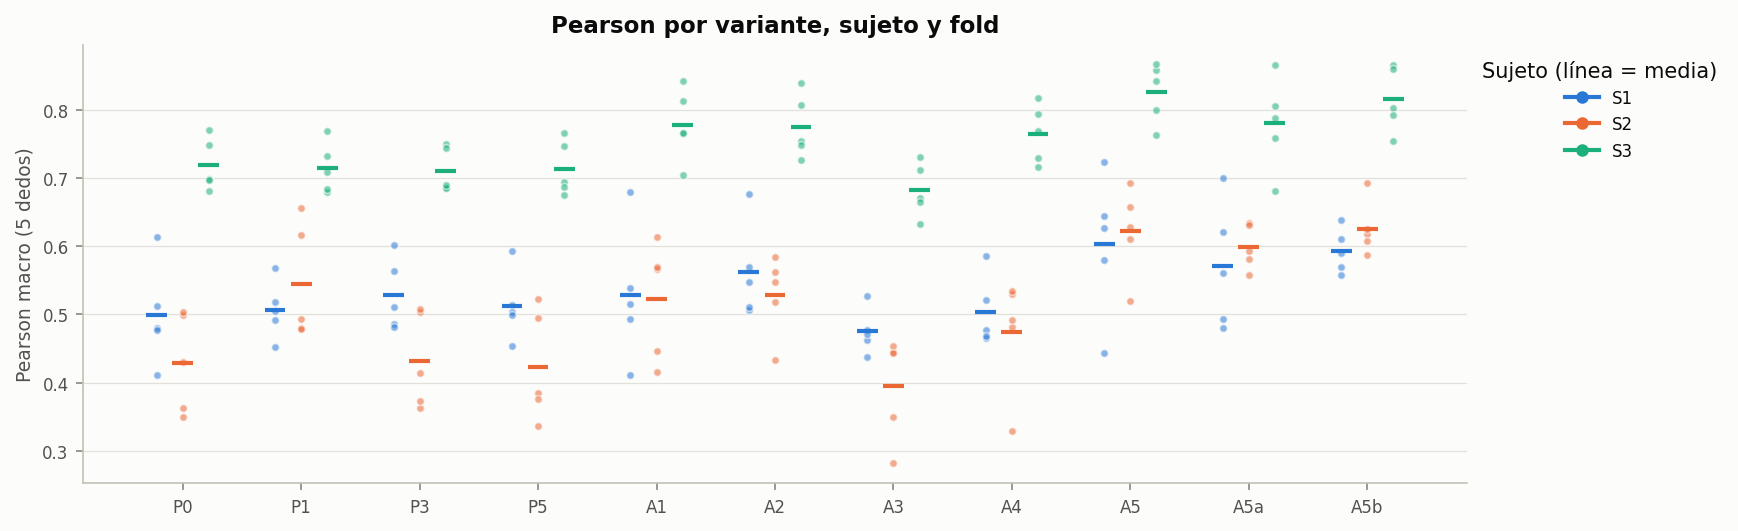
\includegraphics[width=0.95\linewidth,height=0.35\textheight,keepaspectratio]{imgs/pearson_by_variant.png}\\
      {\tiny \textbf{(a)} Correlaci\'on de Pearson macro por variante en validaci\'on cruzada (\'epoca 50).}\\[1mm]
      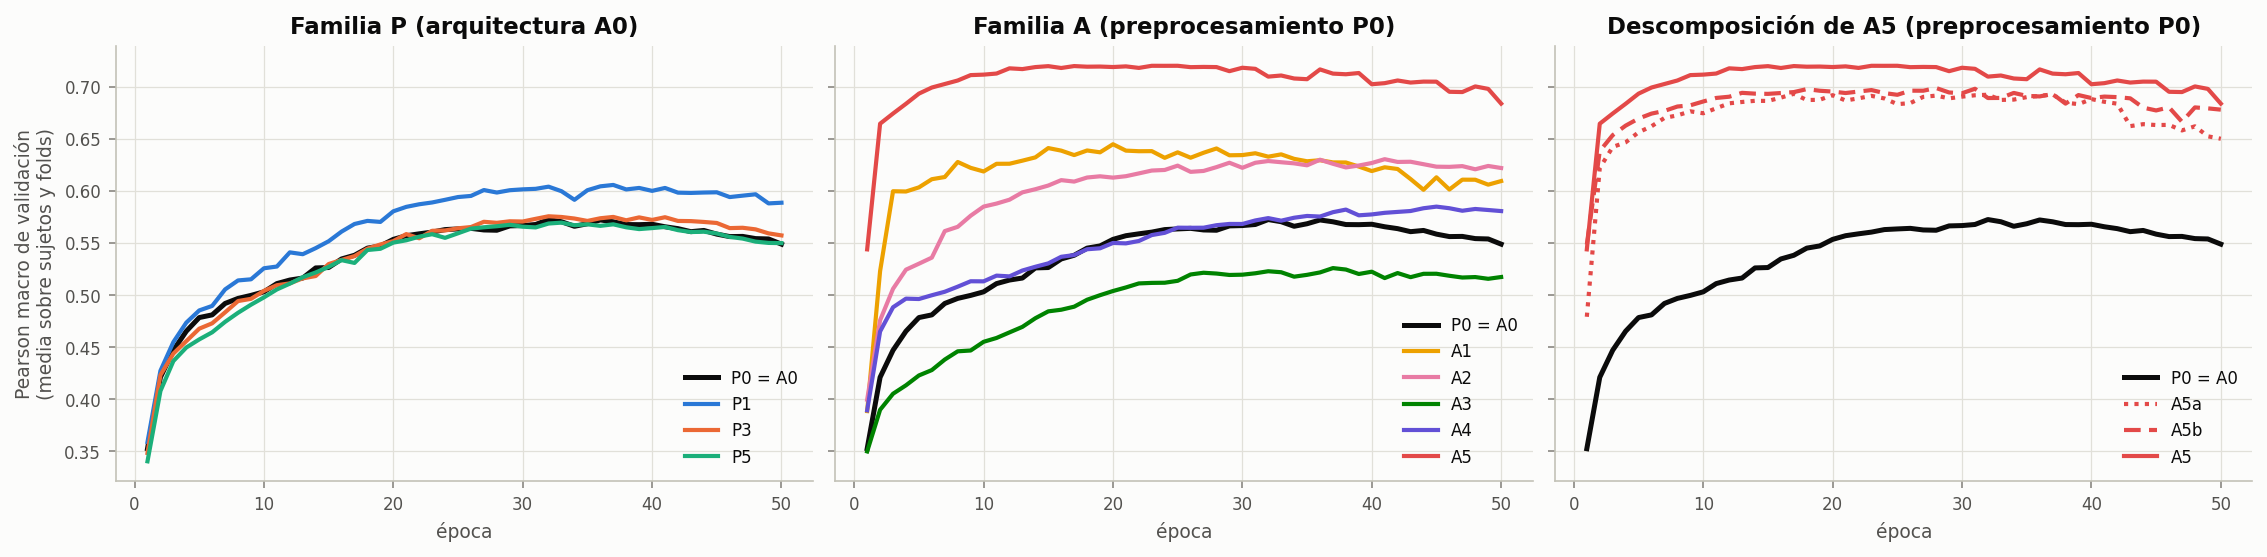
\includegraphics[width=0.95\linewidth,height=0.35\textheight,keepaspectratio]{imgs/training_curves.png}\\
      {\tiny \textbf{(b)} Din\'amica de convergencia y brecha entre mejor \textit{checkpoint} y \'epoca 50.}
    \end{column}
  \end{columns}
\end{frame}

% --- DIAPOSITIVA 11: ETAPAS 3 Y 4: BÚSQUEDA TPE, VERIFICACIÓN Y MODELOS ELEGIDOS ---
\begin{frame}{Etapas 3 y 4: B\'usqueda TPE, Verificaci\'on Multi-Semilla y Modelos Elegidos}{Control del sesgo de selecci\'on y configuraciones finales por sujeto \cite{cawley2010overfitting,rodas_valencia_tpe_ecog}}
  \begin{columns}[T,onlytextwidth]
    \begin{column}{0.54\textwidth}
      \scriptsize
      \begin{block}{Separaci\'on Rigurosa de Efectos en CV}
        \begin{itemize}\setlength{\itemsep}{2pt}
          \item \textbf{B\'usqueda TPE (Etapa 3, $480$ fits):} El salto aparente de $0.6837$ a $0.7509$ ($+0.0672$) se descompone en $\mathbf{+0.0493}$ por el criterio de \textit{checkpoint} y $\mathbf{+0.0179}$ por la b\'usqueda TPE (\texttt{S2} sube $+0.0413$).
          \item \textbf{Verificaci\'on multi-semilla (Etapa 4, $60$ fits con semillas nuevas):}
            \begin{itemize}\scriptsize
              \item \texttt{A5} ($\mathbf{0.7372}$) supera consistentemente a \texttt{A5b} ($0.7112$, $\mathbf{\Delta = +0.0260}$) en los 3 sujetos.
              \item Frente a \texttt{A5} sin TPE con \textit{checkpoint} ($0.7330$), el beneficio global verificado es marginal ($\mathbf{+0.0041}$), pero \textbf{se conserva una mejora sustancial en \texttt{S2} ($\mathbf{+0.0319}$)}.
            \end{itemize}
        \end{itemize}
      \end{block}

      \centering
      \renewcommand{\arraystretch}{1.15}
      \setlength{\tabcolsep}{3pt}
      {\tiny
      \begin{tabular}{@{} l c c c c c c @{}}
        \toprule
        \rowcolor{ipnDark}
        \textcolor{white}{\textbf{Sujeto (Trial)}} &
        \textcolor{white}{\textbf{$k, L, f$}} &
        \textcolor{white}{\textbf{Params}} &
        \textcolor{white}{\textbf{LR ($\eta$)}} &
        \textcolor{white}{\textbf{$L_2$ ($\lambda$)}} &
        \textcolor{white}{\textbf{Verif.\ CV}} &
        \textcolor{white}{\textbf{\'Ep.\ Test (\texttt{B1--B5})}} \\
        \midrule
        \textbf{\texttt{S1}} (Trial 10) & $5, 5, 64$ & $9.35\text{ M}$ & $1.38\times 10^{-4}$ & $6.27\times 10^{-7}$ & $0.6929$ & \textbf{21 \'epocas} \\
        \rowcolor{rowHighlight}
        \textbf{\texttt{S2}} (Trial 30) & $7, 5, 96$ & $28.03\text{ M}$ & $5.16\times 10^{-5}$ & $4.35\times 10^{-6}$ & $0.6785$ & \textbf{32 \'epocas} \\
        \textbf{\texttt{S3}} (Trial 26) & $7, 5, 64$ & $12.71\text{ M}$ & $5.10\times 10^{-5}$ & $1.23\times 10^{-7}$ & $0.8402$ & \textbf{28 \'epocas} \\
        \bottomrule
      \end{tabular}}
    \end{column}

    \begin{column}{0.44\textwidth}
      \centering
      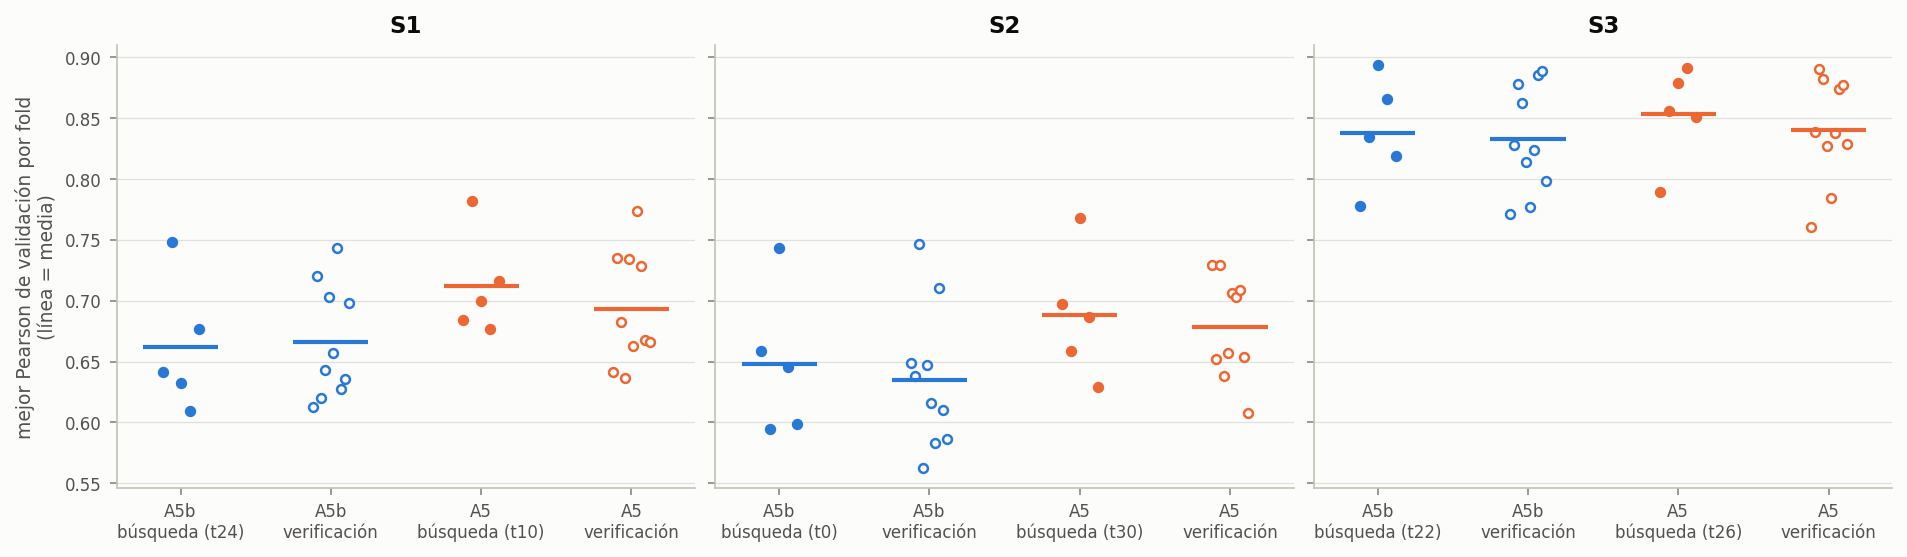
\includegraphics[width=\linewidth,height=0.55\textheight,keepaspectratio]{imgs/verification.png}\\[1mm]
      \begin{beamercolorbox}[wd=\linewidth,rounded=true,sep=1.8mm]{block body alerted}
        \tiny
        \textbf{Regla anti-\textit{leakage} para Test:} La mediana de \'epocas \'optimas en las $10$ corridas de verificaci\'on ($21, 32, 28$) fija la duraci\'on del reentrenamiento \texttt{B1--B5} sin tocar jam\'as el bloque de prueba \cite{cawley2010overfitting}.
      \end{beamercolorbox}
    \end{column}
  \end{columns}
\end{frame}

% --- DIAPOSITIVA 12: ETAPA 5: EVALUACIÓN EN TEST OFICIAL Y DESGLOSE POR DEDO ---
\begin{frame}{Etapa 5: Evaluaci\'on en el Conjunto de Prueba Oficial y Desglose por Dedo}{Desempe\~no final auditado en las 3 semillas (\texttt{3042, 4042, 5042}) \cite{lin1989concordance,rodas_valencia_tpe_ecog}}
  \begin{columns}[T,onlytextwidth]
    \begin{column}{0.52\textwidth}
      \scriptsize
      \centering
      \renewcommand{\arraystretch}{1.16}
      \setlength{\tabcolsep}{3.5pt}
      \begin{tabular}{@{} l c c c c @{}}
        \toprule
        \rowcolor{ipnDark}
        \textcolor{white}{\textbf{Sujeto}} &
        \textcolor{white}{\textbf{Test Inicial (\texttt{B1--B4})}} &
        \textcolor{white}{\textbf{Pearson Test (\texttt{B1--B5})}} &
        \textcolor{white}{\textbf{CCC de Lin}} &
        \textcolor{white}{\textbf{MSE}} \\
        \midrule
        \textbf{\texttt{S1}} & $0.6087 \pm 0.0110$ & $\mathbf{0.6723 \pm 0.0009}$ & $0.5534$ & $0.6497$ \\
        \rowcolor{rowLight}
        \textbf{\texttt{S2}} & $0.5226 \pm 0.0033$ & $\mathbf{0.5490 \pm 0.0143}$ & $0.4050$ & $0.8667$ \\
        \textbf{\texttt{S3}} & $0.7685 \pm 0.0040$ & $\mathbf{0.7796 \pm 0.0069}$ & $0.7694$ & $0.3606$ \\
        \midrule
        \rowcolor{rowHighlight}
        \textbf{Media} & $\mathbf{0.6333}$ & $\mathbf{0.6669}$ ($\mathbf{+0.0337}$) & $\mathbf{0.5759}$ & $\mathbf{0.6257}$ \\
        \bottomrule
      \end{tabular}

      \vspace{1.5mm}
      \begin{block}{Comparaci\'on Transparente de Protocolos y Dedos}
        \begin{itemize}\scriptsize\setlength{\itemsep}{2pt}
          \item \textbf{Protocolo \texttt{b1b4\_es\_b5} ($0.6333$) $\to$ \texttt{b1b5\_fixed} ($0.6669$):} Reentrenar con los 5 bloques mejora Pearson en las \textbf{$9/9$ parejas sujeto-semilla} (se reportan ambas cifras por transparencia).
          \item \textbf{Ranking por dedo (\texttt{b1b5\_fixed}):}
            \begin{enumerate}\tiny
              \item \textbf{Anular:} $\mathbf{0.7202}$ ($\text{S1}=0.7429, \text{S2}=0.6431, \text{S3}=0.7745$)
              \item \textbf{\'Indice:} $\mathbf{0.7161}$ ($\text{S1}=0.7525, \text{S2}=0.6197, \text{S3}=0.7760$)
              \item \textbf{Pulgar:} $\mathbf{0.6914}$ \,|\, \textbf{Me\~nique:} $\mathbf{0.6328}$
              \item \textbf{Medio:} $\mathbf{0.5742}$ (mayor coactivaci\'on biomec\'anica; $\text{S2}=0.4107$).
            \end{enumerate}
        \end{itemize}
      \end{block}
    \end{column}

    \begin{column}{0.46\textwidth}
      \centering
      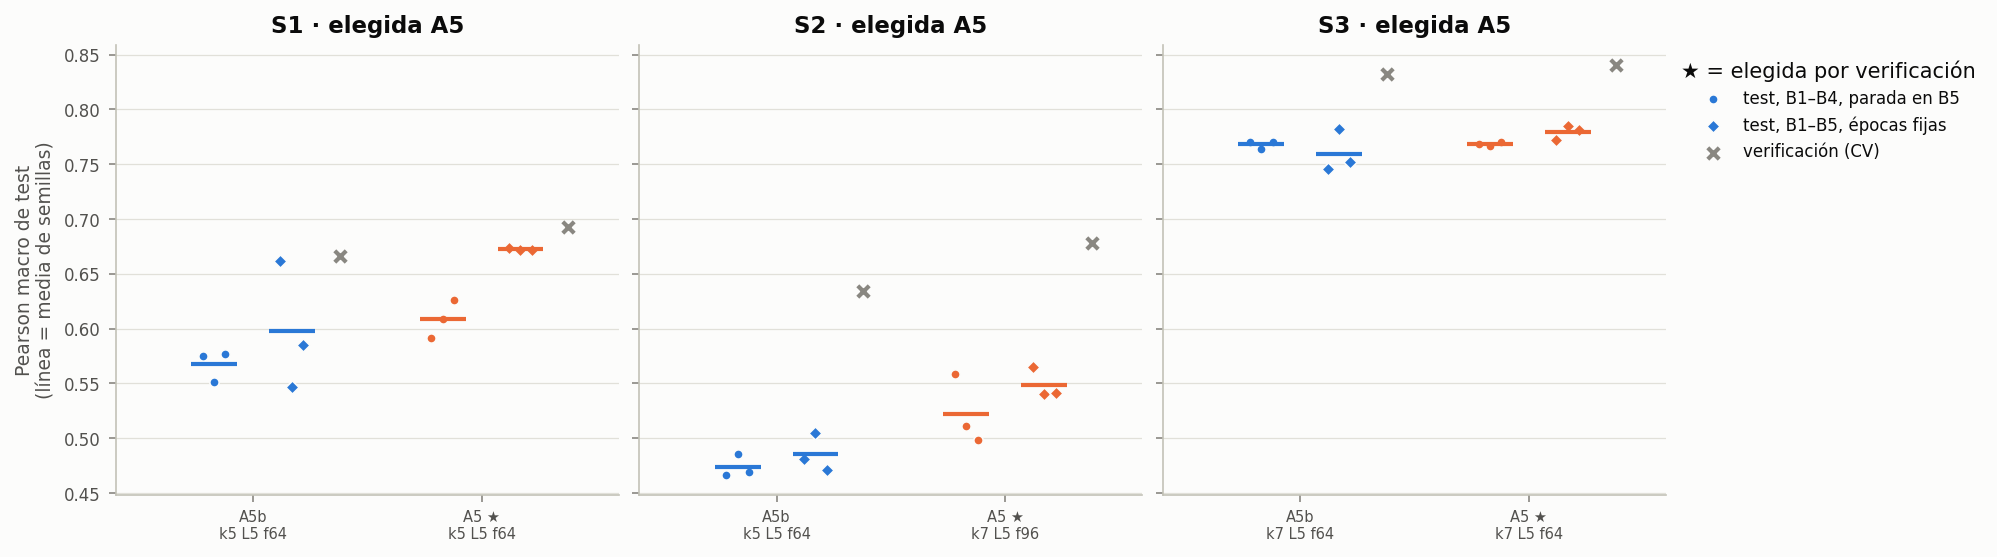
\includegraphics[width=0.95\linewidth,height=0.35\textheight,keepaspectratio]{imgs/test_scores.png}\\
      {\tiny \textbf{(a)} Comparaci\'on en Test Oficial: \texttt{b1b4\_es\_b5} ($0.6333$) vs.\ \texttt{b1b5\_fixed} ($0.6669$).}\\[1mm]
      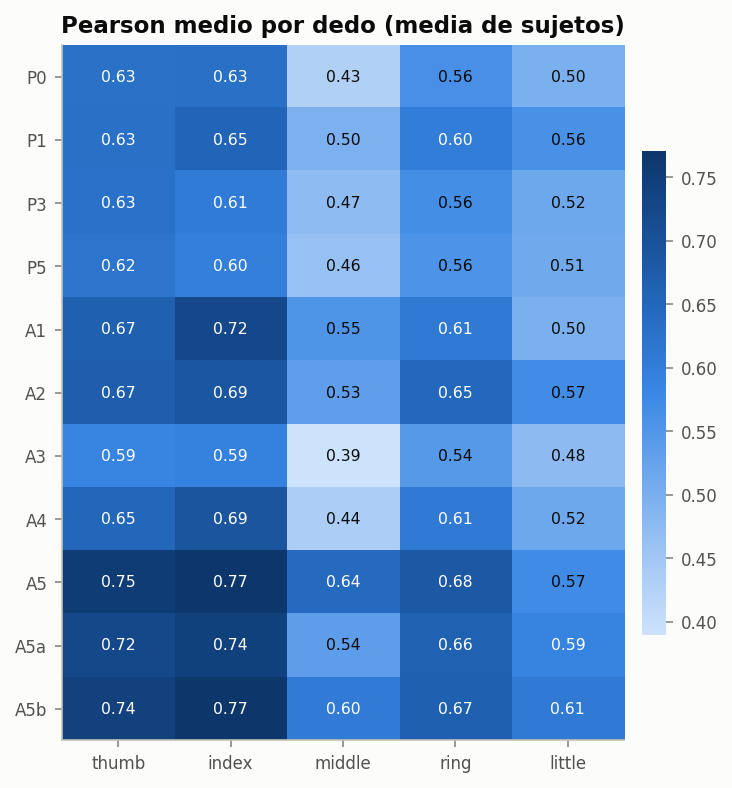
\includegraphics[width=0.95\linewidth,height=0.35\textheight,keepaspectratio]{imgs/pearson_per_finger.png}\\
      {\tiny \textbf{(b)} Desempe\~no desglosado por dedo: liderazgo en Anular e \'Indice.}
    \end{column}
  \end{columns}
\end{frame}

% --- DIAPOSITIVA 13: DEMOSTRACIÓN DE TRAYECTORIAS Y AUDITORÍA V01-V14 ---
\begin{frame}{Demostraci\'on del Sistema: Trayectorias Continuas y Auditor\'ia \texttt{V01--V14}}{Contraste visual del seguimiento cinem\'atico e ingenier\'ia de software reproducible}
  \begin{columns}[T,onlytextwidth]
    \begin{column}{0.49\textwidth}
      \centering
      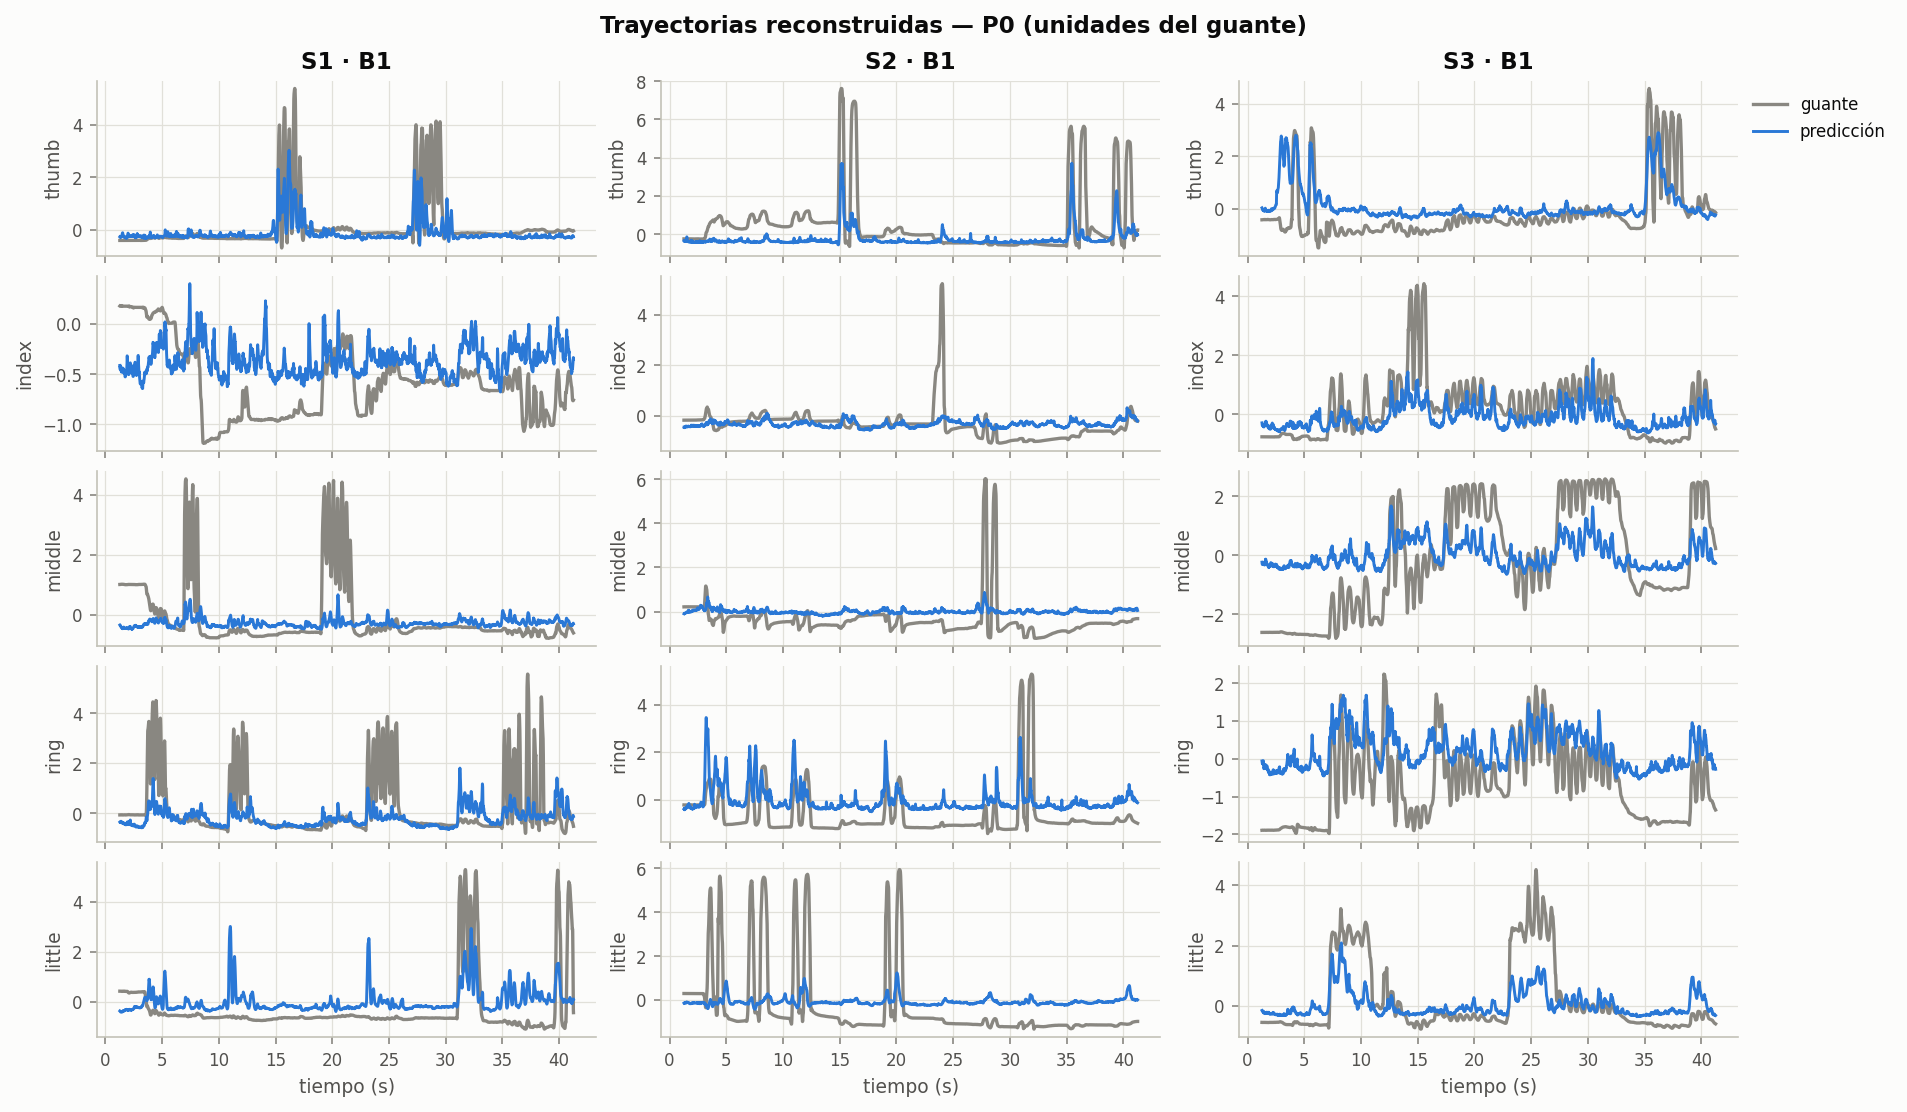
\includegraphics[width=\linewidth,height=0.45\textheight,keepaspectratio]{imgs/example_predictions_P0.png}\\
      {\tiny \textbf{(a) Modelo Base \texttt{A0/P0} ($0.5489$ CV):} fluctuaciones de alta frecuencia y menor ajuste de amplitud.}
    \end{column}
    \begin{column}{0.49\textwidth}
      \centering
      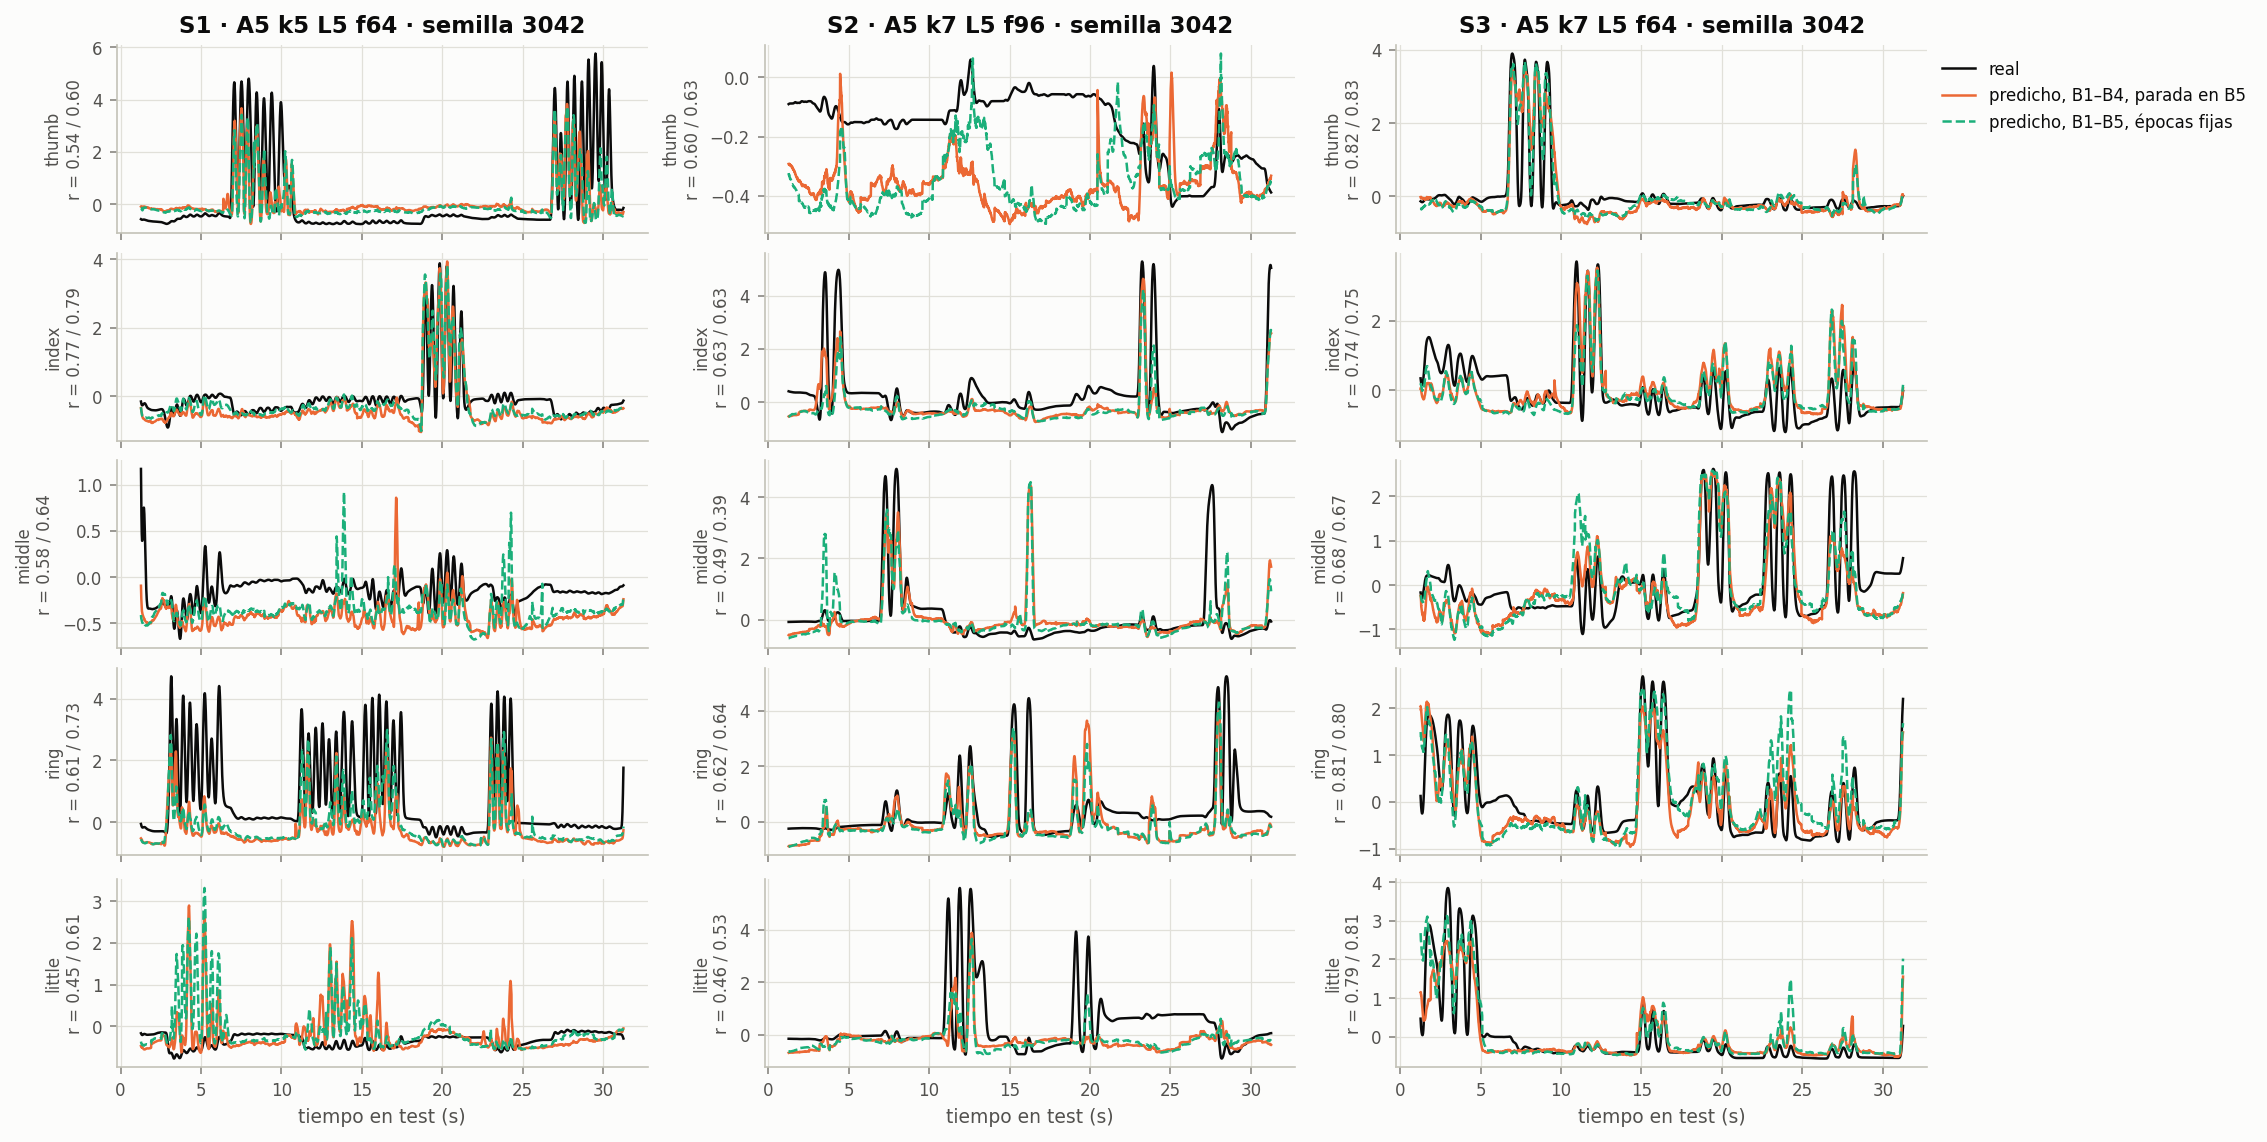
\includegraphics[width=\linewidth,height=0.45\textheight,keepaspectratio]{imgs/test_trajectories.png}\\
      {\tiny \textbf{(b) Nuestro Modelo \texttt{A5} en Test Oficial ($0.6669$):} captura precisa de envolventes, silencios y retornos a reposo.}
    \end{column}
  \end{columns}

  \vspace{1.5mm}
  \begin{alertblock}{Ingenier\'ia de Software Reproducible y Auditor\'ia Automatizada (\texttt{V01--V14})}
    \scriptsize
    \begin{itemize}\setlength{\itemsep}{1.5pt}
      \item \textbf{Trazabilidad criptogr\'afica:} Manifiesto congelado \texttt{frozen.json} con hash SHA-256 (\texttt{pipeline\_id: b26db4c45dc16388...}) y ejecuci\'on transaccional en GPU NVIDIA A100 con reanudaci\'on at\'omica.
      \item \textbf{14 Compuertas de Verificaci\'on (\texttt{14/14 PASS}):} Validan soporte exacto de bordes ($\pm 125\text{ muestras}$), ausencia absoluta de solapamiento con tolerancia $\mathbf{0.0}$ entre train/val/test, ajuste exclusivo de escaladores en train y paridad de semillas en Optuna TPE.
    \end{itemize}
  \end{alertblock}
\end{frame}

% --- DIAPOSITIVA 14: COMPARACIÓN CRÍTICA FRENTE AL ESTADO DEL ARTE (OP4) ---
\begin{frame}{Comparaci\'on Cr\'itica frente al Estado del Arte (Objetivo Particular 4)}{Posicionamiento en el benchmark \textit{BCI Competition IV Dataset 4} \cite{liang2012decoding,Lomtev2022,wang2025dtcnet,rodas_valencia_tpe_ecog}}
  \begin{columns}[T,onlytextwidth]
    \begin{column}{0.53\textwidth}
      \centering
      \tiny
      \renewcommand{\arraystretch}{1.18}
      \setlength{\tabcolsep}{3pt}
      \begin{tabular}{@{} l c c c c @{}}
        \toprule
        \rowcolor{ipnDark}
        \textcolor{white}{\textbf{M\'etodo / Arquitectura en Literatura}} &
        \textcolor{white}{\textbf{S1}} &
        \textcolor{white}{\textbf{S2}} &
        \textcolor{white}{\textbf{S3}} &
        \textcolor{white}{\textbf{Promedio}} \\
        \midrule
        \textit{Switching linear model} (Liang \& Bougrain, 2012) \cite{liang2012decoding} & $0.48$ & $0.24$ & $0.56$ & $0.43$ \\
        \rowcolor{rowLight}
        \textit{Compact CNN} (2018) / \textit{Linear regression} (2017) & $0.45$ & $0.34$ & $0.56$ & $0.45\text{--}0.48$ \\
        \textit{CNN-LSTM} (Xie et al., 2018) / \textit{Multi purpose CNN} (2021) & $0.56$ & $0.41$ & $0.58$ & $0.52$ \\
        \rowcolor{rowLight}
        \textit{highGRM} (2022) & $0.55$ & $0.42$ & $0.61$ & $0.53$ \\
        \midrule
        \textbf{\textit{FingerFlex}} (U-Net 1D, Lomtev et al., 2022) \cite{Lomtev2022} & $0.64$ & $0.56$ & $0.73$ & $\mathbf{0.64}$ \\
        \rowcolor{rowLight}
        \textbf{\textit{DTCNet}} (Conv 3D dilatada, Wang et al., 2025) \cite{wang2025dtcnet} & $0.71$ & $0.59$ & $0.77$ & $\mathbf{0.69}$ \\
        \midrule
        \textbf{Nuestro \texttt{A0/P0}} (Base TT1, CV \'ep.\ 50) & $0.4990$ & $0.4289$ & $0.7187$ & $0.5489$ \\
        \rowcolor{rowLight}
        \textbf{Nuestro \texttt{A5}} (Test inicial \texttt{b1b4\_es\_b5}, 3 semillas) & $0.6087$ & $0.5226$ & $0.7685$ & $\mathbf{0.6333}$ \\
        \rowcolor{rowHighlight}
        \textbf{Nuestro \texttt{A5}} (Test reentrenado \texttt{b1b5\_fixed}, 3 semillas) & $\mathbf{0.6723}$ & $\mathbf{0.5490}$ & $\mathbf{0.7796}$ & $\mathbf{0.6669}$ \\
        \bottomrule
      \end{tabular}
    \end{column}

    \begin{column}{0.45\textwidth}
      \scriptsize
      \begin{block}{Hallazgos Clave de la Comparaci\'on}
        \begin{enumerate}\setlength{\itemsep}{2.5pt}
          \item \textbf{Superaci\'on de \textit{FingerFlex} \cite{Lomtev2022}:} Nuestro modelo \texttt{A5} ($0.6669$) supera al referente directo U-Net 1D ($0.64$) en \textbf{\texttt{S1} ($+0.0323$), \texttt{S3} ($+0.0496$) y en la media global ($\mathbf{+0.0269}$)}.
          \item \textbf{Contraste granular frente a \textit{DTCNet} \cite{wang2025dtcnet}:} Aunque \textit{DTCNet} (que proyecta la rejilla a tensores 3D) reporta $0.69$ global, nuestra red 1D \texttt{A5} \textbf{lo supera en el Sujeto 3 ($0.7796$ vs.\ $0.77$), en el promedio del dedo Anular ($0.7202$ vs.\ $0.70$) y en $8\text{ de los }15$ pares sujeto-dedo}; la brecha se concentra en el dedo Medio ($0.5742$ vs.\ $0.67$).
          \item \textbf{Rigor de comparabilidad:} Contraste contextual; reportamos el promedio estricto de 3 semillas auditadas (\texttt{V01--V14}).
        \end{enumerate}
      \end{block}
    \end{column}
  \end{columns}
\end{frame}
